\section{Proposed Method}

% -------------------------------------------------------------------------
% FIGURE 1: UNIFIED ARCHITECTURE DIAGRAM (Combines Pipeline, I/O, & Smooth L1)
% Spans both columns using \begin{figure*}
% -------------------------------------------------------------------------
\begin{figure*}[t]
    \centering
    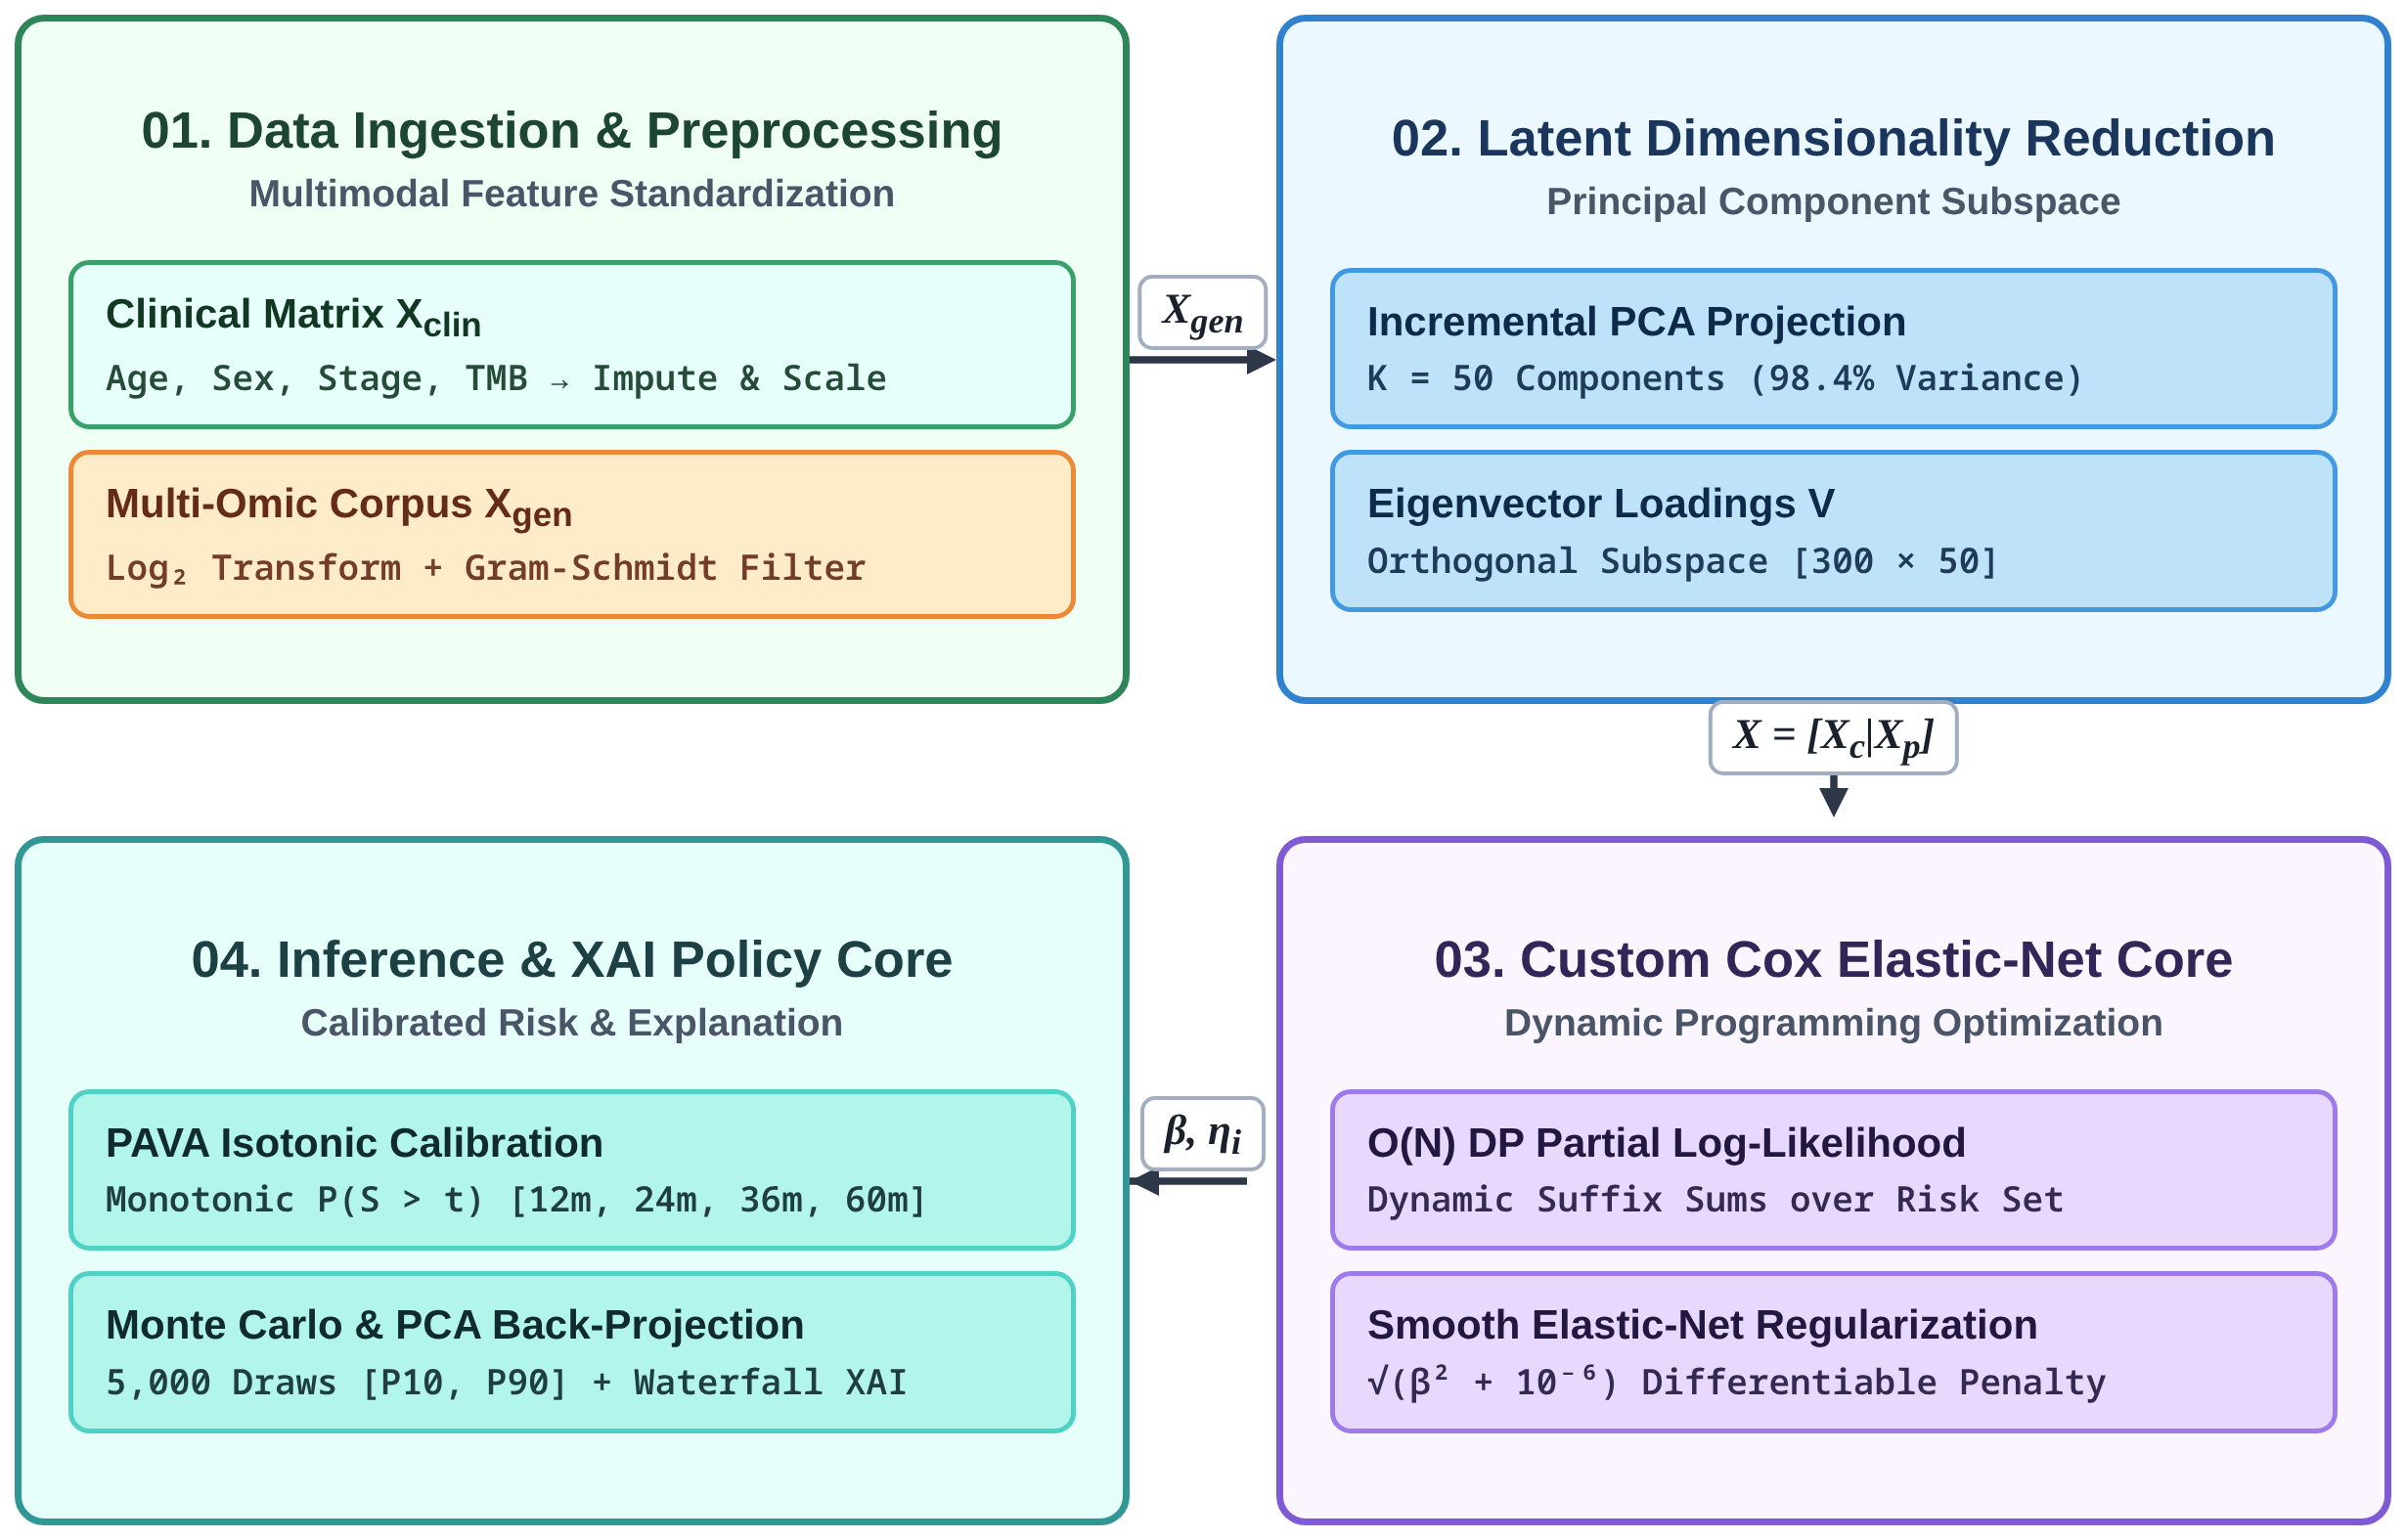
\includegraphics[width=\textwidth]{images/fig1_unified_architecture.png}
    \caption{Unified multi-omic survival analysis pipeline, component input matrices, and smooth Elastic-Net optimization architecture.}
    \label{fig:unified_architecture}
\end{figure*}

\subsection{Feature Preprocessing \& Standardized Latent Principal Component Projection}
We isolate $P_{\text{raw}} = 300$ high-variance genes [2] from the overarching expression corpus to evade the $P \gg N$ dimensionality trap. Linear models suffer optimization failures when they process parallel feature vectors. We implement an incremental Gram-Schmidt orthogonalization pass [1] to drop redundant transcripts. The algorithm computes the cosine similarity between each incoming gene vector and the preserved subspace. We reject any new gene demonstrating a correlation magnitude exceeding $0.75$. This dynamic filter scales in $O(N \cdot P_{\text{raw}})$ time and avoids the $O(N^3)$ memory overhead required for full Variance Inflation Factor matrix inversion. Following collinearity reduction, we apply a base-two logarithmic transformation to the raw gene expression matrix $G \in \mathbb{R}^{N \times 300}$ [6] to compress right-skewed negative binomial read counts. We add a pseudocount of one to prevent undefined operations at zero. We standardize the result to zero mean and unit variance, producing the scaled matrix $Z_{\text{gene}} \in \mathbb{R}^{N \times 300}$. Principal Component Analysis [1] isolates the axes of maximum biological variance. We compute the right-singular eigenvector loading matrix $V \in \mathbb{R}^{300 \times 50}$ where $V^T V = I_{50}$ via singular value decomposition. We project the standardized genes onto $K = 50$ latent dimensions [2] to yield the dense genomic feature matrix $X_{\text{pca}} = Z_{\text{gene}} V \in \mathbb{R}^{N \times 50}$. The overarching data ingestion and feature projection workflow operates as illustrated in the initial stages of Figure~\ref{fig:unified_architecture}.

\subsection{Unified Model Input Feature Matrix \& Cox Elastic-Net Partial Log-Likelihood}
We format the clinical data through an initial preprocessing phase to integrate it with the transcriptomic profiles. The pipeline targets numeric variables like age and tumor mutational burden alongside categorical indicators such as tumor stage and patient sex. We process categorical fields using one-hot encoding while dropping the first column to prevent collinear dummy variable traps. We apply median imputation to missing continuous clinical values to resist outlier skew. We impute missing expression data with zero to reflect undetected transcripts. We scale these structured variables to output the clinical feature matrix $X_{\text{clin}} \in \mathbb{R}^{N \times 9}$. We concatenate the biological and clinical modalities into a single input feature matrix $X = [X_{\text{clin}} \mid X_{\text{pca}}] \in \mathbb{R}^{N \times 59}$. Figure~\ref{fig:unified_architecture} details these matrix dimension transformations from the initial $[N \times 305]$ input to the final $[N \times 1]$ target vector. The Cox proportional hazards model [3] generates a continuous relative risk score $\eta_i = X_i \beta$ for each patient $i$, where the coefficient vector is $\beta = [\beta_{\text{clin}} \mid \beta_{\text{pca}}] \in \mathbb{R}^{59}$. The foundational hazard function is $h(t \mid X_i) = h_0(t) \exp(\eta_i)$. The standard Breslow partial log-likelihood calculation [7] requires an $O(N^2)$ nested loop to evaluate the risk set at each failure time. We sort the event times in descending order to engineer an $O(N)$ dynamic programming solution. We compute suffix sums $S^{(0)}(t_i)$ and $S^{(1)}(t_i)$ over the exponentiated risk scores to evaluate the risk-set denominator in a single contiguous memory pass.

\subsection{Smooth Elastic-Net Regularization Objective}
We extract the coefficients representing independent prognostic correlation by minimizing the negative partial log-likelihood. Unpenalized Cox regression [5] fails on high-dimensional medical data. We impose an Elastic-Net penalty [4] combining absolute and squared coefficient constraints to force correlated gene pathways to shrink together while eliminating pure noise elements. We optimize the objective function using the Limited-memory Broyden-Fletcher-Goldfarb-Shanno with Box constraints algorithm. This optimizer approximates the inverse Hessian matrix using a bounded memory cache to conserve computational resources. The pure L1 penalty poses a mathematical barrier because the absolute value function creates a non-differentiable kink at zero. This sharp vertex forces the gradient solver to crash. We inject a continuous scalar approximation $\sqrt{\beta^2 + \epsilon}$ into the objective. Figure~\ref{fig:unified_architecture} visualizes this mathematical comparison, demonstrating how the injected epsilon factor grants differentiability at zero to prevent solver failures. We set the epsilon smoothing factor [3] to $\epsilon = 10^{-6}$. This hyperparameter value preserves the feature selection properties of the penalty while granting the gradient vector a smooth curve to traverse through zero. We bound the linear predictor $\eta_i$ to the interval $[-40, 40]$ prior to exponentiation to evade float64 infinity overflow limits during the Hessian evaluation.

\subsection{Isotonic Calibration \& Inverse Transform Monte Carlo Simulation}
The uncalibrated risk scalar $\eta_i$ provides arbitrary relative hazard ratios that hold little value for immediate clinical planning. We convert these unitless outputs into definitive probability bounds across fixed time horizons [8]. We isolate a separate calibration fold before any feature selection or scaling takes place. We fit a non-parametric Isotonic Regression model using the Pool Adjacent Violators Algorithm to output the monotonic calibration function $f_{\text{iso},t}(\eta_i)$. This function maps the raw risk scores to absolute survival probabilities $P(S > t \mid \eta_i)$ evaluated at $t \in \{12, 24, 36, 60\}$ months, mapping empirical Kaplan-Meier survival rates. Beyond point estimates, we quantify temporal uncertainty by simulating distinct patient trajectories across the underlying cumulative baseline hazard $\Lambda_0(t)$ [7]. We implement an inverse transform Monte Carlo sampling loop to generate a distribution of possible life spans (Figure~\ref{fig:inference_xai_architecture}). The engine draws $5,000$ independent uniform random variables $U^{(k)} \sim \text{Uniform}(0, 1)$ per patient. We map each draw against the inverted baseline hazard scaled by the exponentiated relative risk. We search the step-function array using a binary search algorithm to locate the exact simulated month of mortality. We aggregate these iterations to establish the pessimistic $P10$, median $P50$, and optimistic $P90$ absolute survival bounds in months. We compute the Restricted Mean Survival Time (RMST) capped at $60$ months to evaluate the area under the synthesized survival curve.

% -------------------------------------------------------------------------
% FIGURE 2: INFERENCE ENGINE & XAI POLICY ARCHITECTURE DIAGRAM
% -------------------------------------------------------------------------
\begin{figure}[t]
    \centering
    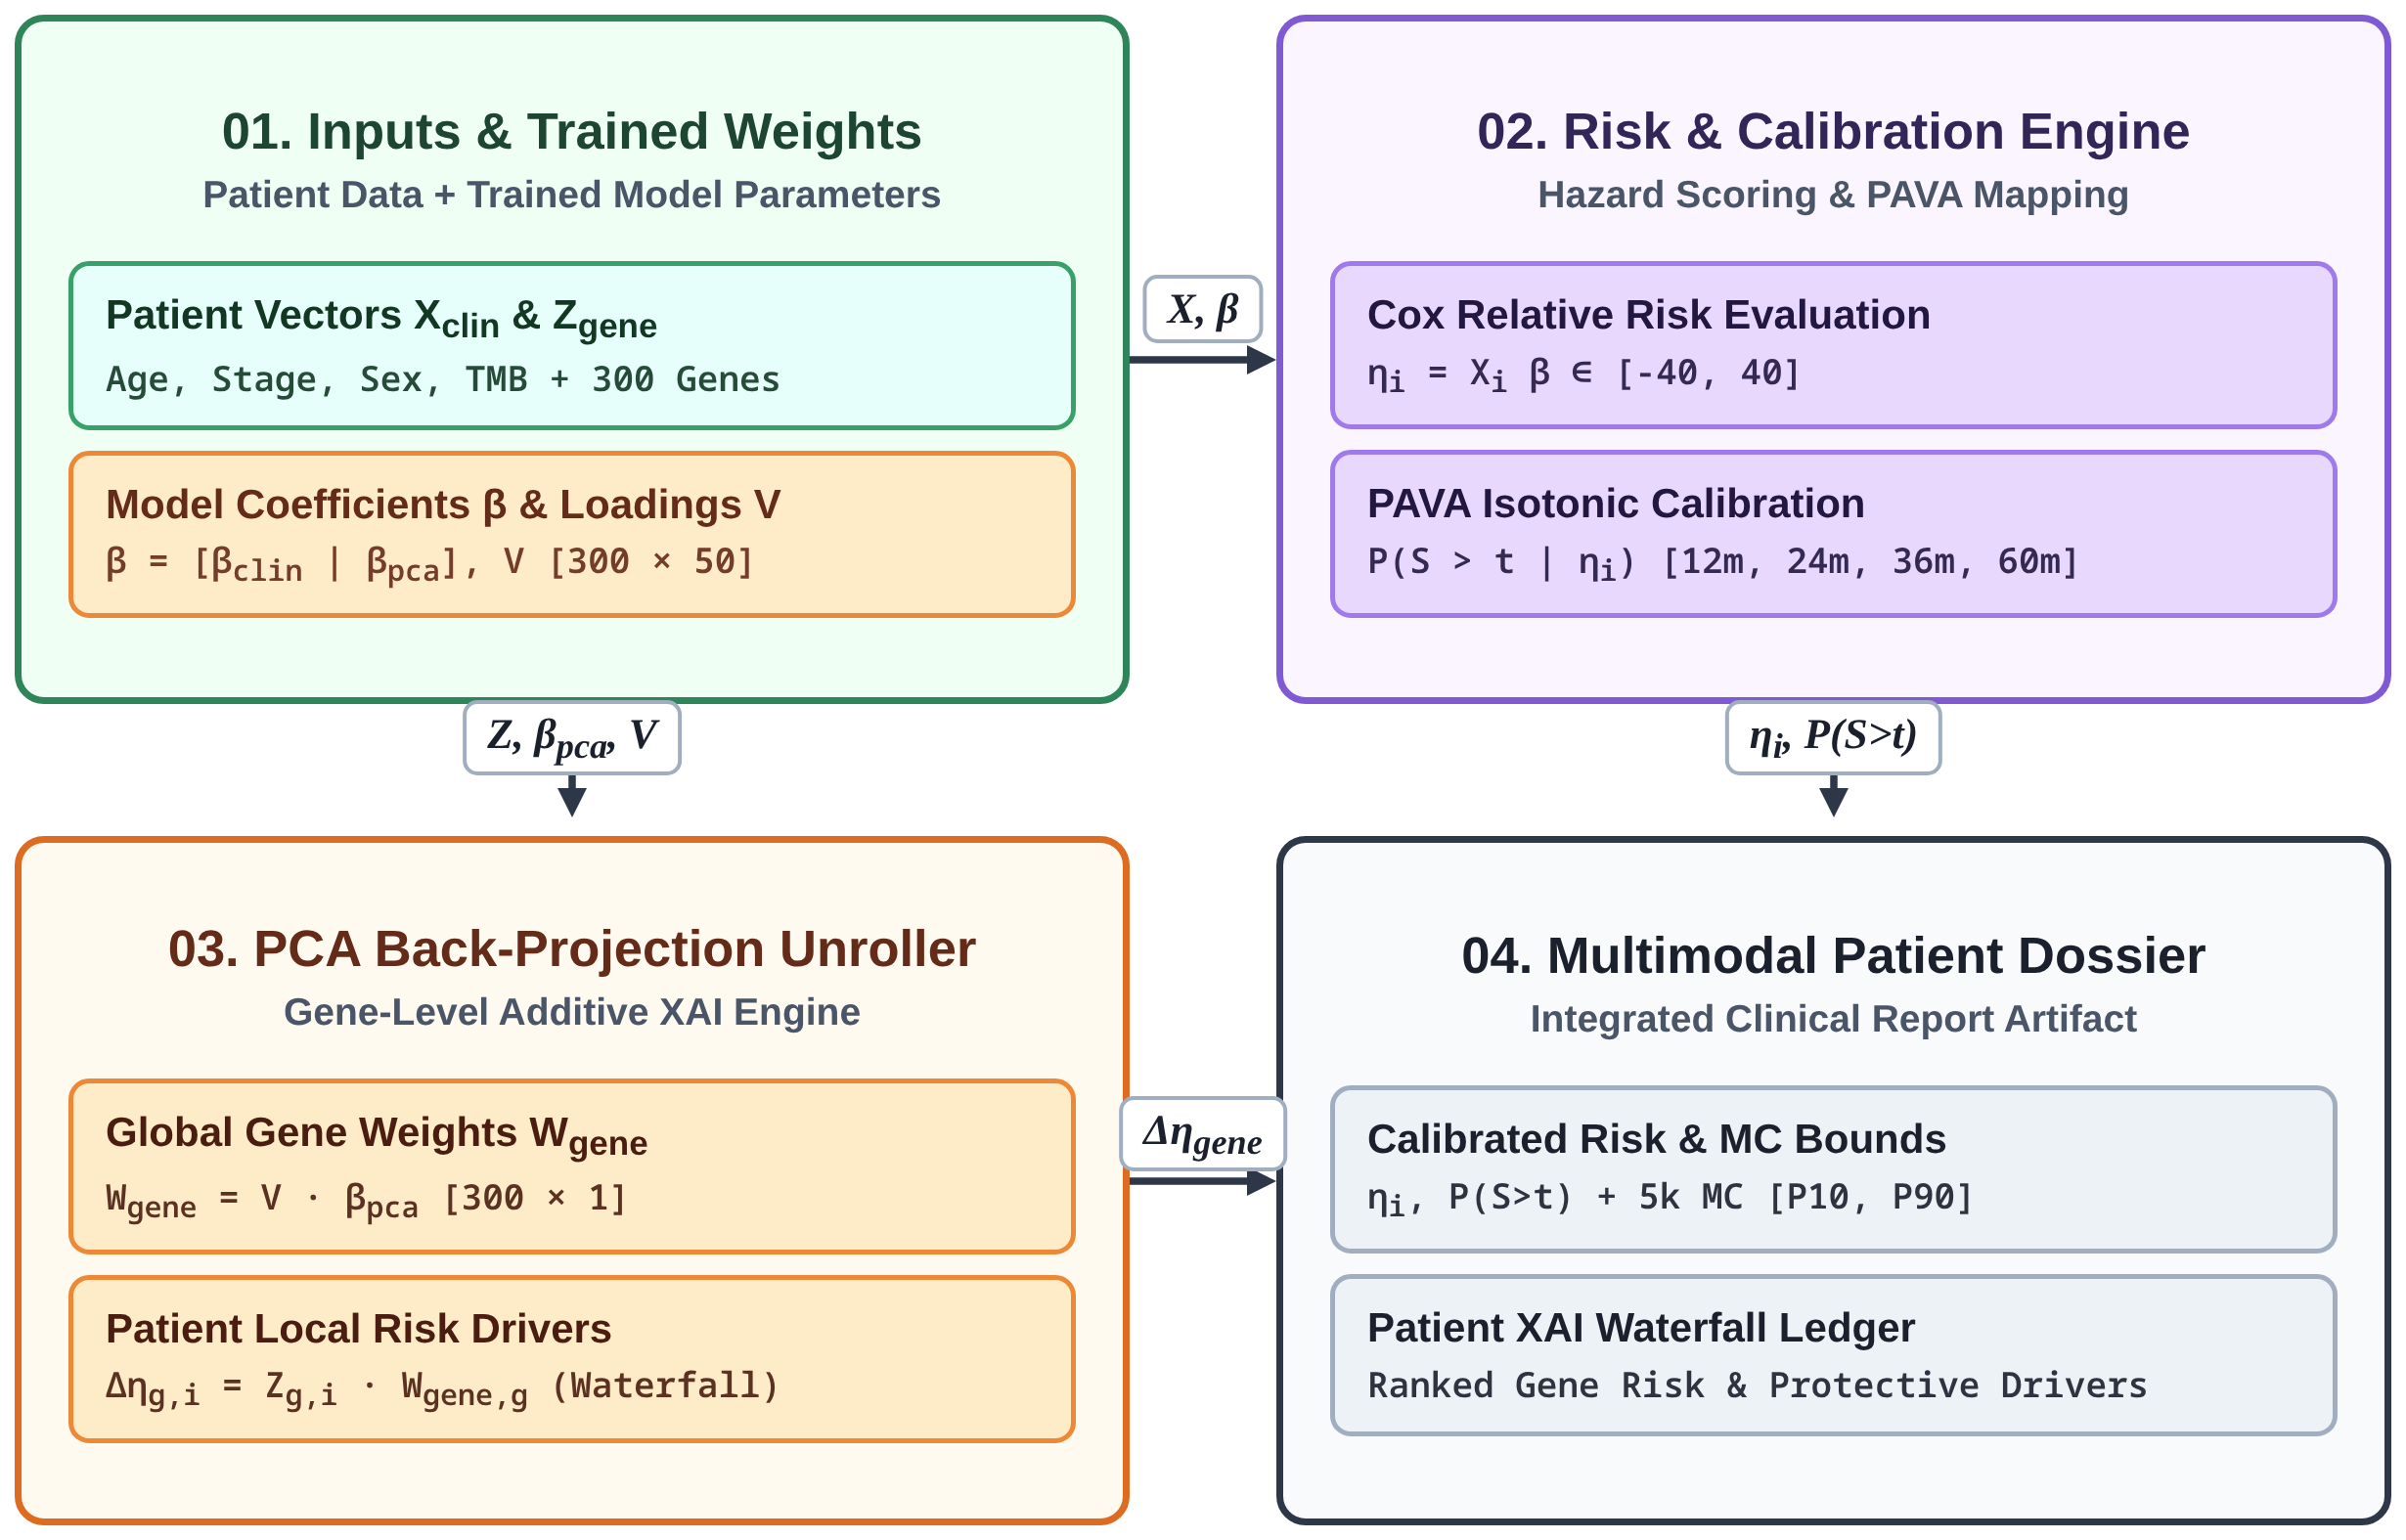
\includegraphics[width=\linewidth]{images/fig2_inference_xai_architecture.png}
    \caption{Architectural data flow of the optimization, inference core, and explainability modules.}
    \label{fig:inference_xai_architecture}
\end{figure}

\subsection{Closed-Form PCA Back-Projection \& Local Patient Risk Waterfall}
Principal Component Analysis [1] compresses raw genetic information into latent orthogonal dimensions. This operation obfuscates the biological mechanisms driving the statistical hazard model. Black-box approximators struggle with the right-censored mathematical architecture inherent to survival datasets. We formulate an exact closed-form matrix operation to unroll the algorithmic compression and map risk weights back to specific oncogenic transcripts. We isolate the subset of the coefficient vector corresponding to the latent dimensions $\beta_{\text{pca}} \in \mathbb{R}^{50}$. We multiply the retained right-singular eigenvector loading matrix $V \in \mathbb{R}^{300 \times 50}$ by these coefficients to yield a global gene risk weight vector $W_{\text{gene}} = V \cdot \beta_{\text{pca}} \in \mathbb{R}^{300}$. This continuous transformation identifies the independent directional impact of each individual transcript. We project the patient-specific standardized expression levels $Z_{g,i}$ against this global vector to compute the local additive risk contribution $\Delta \eta_{g,i} = Z_{g,i} \cdot W_{\text{gene},g}$ for a specific gene $g$. We sort these deterministic scalars to generate unapproximated patient-level waterfall plots detailing the explicit molecular drivers of their assigned mortality score. The unrolled biological vectors operate in tandem with the $9$ standard clinical attributes to provide a unified diagnostic ledger.
